% Original editable schematic for the EUVIP 2026 poster outlook.
% Compile: xelatex -interaction=nonstopmode -halt-on-error foundation-hierarchy.tex
% Size: 15 cm x 5 cm. All labels use explicit 10 pt type at this base size.
\documentclass[tikz,border=0pt]{standalone}
\usepackage{fontspec}
\setmainfont{EB Garamond}
\usepackage{amsmath}
\usetikzlibrary{arrows.meta,calc}
\definecolor{inrianavy}{RGB}{56,66,87}
\definecolor{inriared}{RGB}{230,51,18}
\definecolor{inriablue}{RGB}{20,136,202}
\begin{document}
\fontsize{10}{12}\selectfont
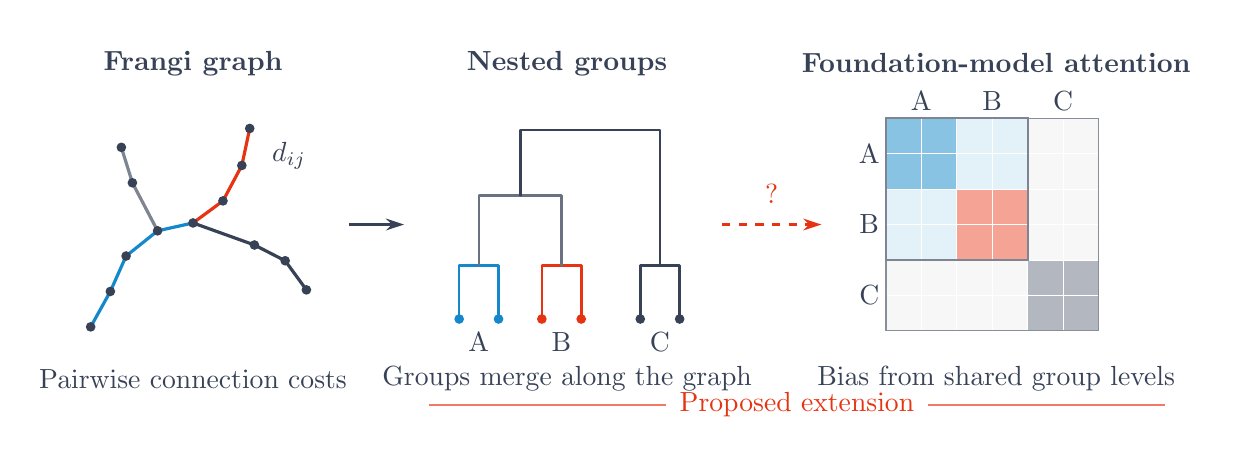
\begin{tikzpicture}[
  x=1cm,y=1cm,
  every node/.style={font=\fontsize{10}{12}\selectfont,text=inrianavy},
  edge/.style={line width=1.15pt,line cap=round,line join=round},
  ridge/.style={circle,inner sep=0pt,minimum size=3.5pt,fill=inrianavy},
  arrow/.style={-{Stealth[length=2.3mm,width=1.5mm]},line width=.9pt,inrianavy},
  branch/.style={line width=.95pt,line cap=round,line join=round}
]
\path[use as bounding box] (0,0) rectangle (15,5);
\fill[white] (0,0) rectangle (15,5);

% Minimal headings; the poster supplies the section title and full caption.
\node[font=\fontsize{10}{12}\selectfont\bfseries] at (2.1,4.55) {Frangi graph};
\node[font=\fontsize{10}{12}\selectfont\bfseries] at (6.85,4.55) {Nested groups};
\node[font=\fontsize{10}{12}\selectfont\bfseries] at (12.3,4.55) {Foundation-model attention};

% 1. A sparse ridge graph, with local edges and a small junction.
\coordinate (g0) at (.8,1.2);
\coordinate (g1) at (1.05,1.65);
\coordinate (g2) at (1.25,2.10);
\coordinate (g3) at (1.65,2.42);
\coordinate (g4) at (2.10,2.52);
\coordinate (g5) at (2.48,2.80);
\coordinate (g6) at (2.72,3.25);
\coordinate (g7) at (2.82,3.72);
\coordinate (g8) at (2.88,2.24);
\coordinate (g9) at (3.27,2.04);
\coordinate (g10) at (3.54,1.67);
\coordinate (g11) at (1.33,3.03);
\coordinate (g12) at (1.19,3.48);
\draw[edge,inriablue] (g0)--(g1)--(g2)--(g3)--(g4);
\draw[edge,inriared] (g4)--(g5)--(g6)--(g7);
\draw[edge,inrianavy] (g4)--(g8)--(g9)--(g10);
\draw[edge,inrianavy!65] (g3)--(g11)--(g12);
\foreach \k in {0,...,12} \node[ridge] at (g\k) {};
\node[anchor=west] at (2.98,3.37) {$d_{ij}$};
\node at (2.1,.54) {Pairwise connection costs};

\draw[arrow] (4.08,2.50)--(4.78,2.50);

% 2. Merge tree: six leaves, three local groups, then coarser unions.
% This is a proposed extension of the EUVIP graph, not an existing output.
\foreach \x in {5.48,5.98} \node[ridge,fill=inriablue] at (\x,1.30) {};
\foreach \x in {6.53,7.03} \node[ridge,fill=inriared] at (\x,1.30) {};
\foreach \x in {7.78,8.28} \node[ridge,fill=inrianavy] at (\x,1.30) {};
\draw[branch,inriablue] (5.48,1.30)--(5.48,1.98)--(5.98,1.98)--(5.98,1.30);
\draw[branch,inriared] (6.53,1.30)--(6.53,1.98)--(7.03,1.98)--(7.03,1.30);
\draw[branch,inrianavy] (7.78,1.30)--(7.78,1.98)--(8.28,1.98)--(8.28,1.30);
\draw[branch,inrianavy!75] (5.73,1.98)--(5.73,2.87)--(6.78,2.87)--(6.78,1.98);
\draw[branch,inrianavy] (6.255,2.87)--(6.255,3.70)--(8.03,3.70)--(8.03,1.98);
\node[fill=white,inner sep=1pt] at (5.73,1.01) {A};
\node[fill=white,inner sep=1pt] at (6.78,1.01) {B};
\node[fill=white,inner sep=1pt] at (8.03,1.01) {C};
\node at (6.85,.54) {Groups merge along the graph};

% The proposed link to a foundation model must remain explicitly uncertain.
\draw[arrow,dashed,inriared] (8.82,2.50)--(10.08,2.50);
\node[text=inriared,fill=white,inner sep=2pt] at (9.45,2.89) {?};

% 3. Illustrative additive bias, not a measured attention heatmap.
% Fine groups occupy 2x2 blocks; A and B share a coarser, weaker block.
\begin{scope}[shift={(10.9,1.15)},x=.45cm,y=.45cm]
  \fill[inrianavy!4] (0,0) rectangle (6,6);
  \fill[inriablue!12] (0,2) rectangle (4,6);
  \fill[inriablue!50] (0,4) rectangle (2,6);
  \fill[inriared!45] (2,2) rectangle (4,4);
  \fill[inrianavy!38] (4,0) rectangle (6,2);
  \draw[step=1,line width=.25pt,white] (0,0) grid (6,6);
  \draw[line width=.45pt,inrianavy!60] (0,0) rectangle (6,6);
  \draw[line width=.8pt,inrianavy!65] (0,2) rectangle (4,6);
  \foreach \x/\label in {1/A,3/B,5/C} {
    \node at (\x,6.48) {\label};
  }
  \foreach \y/\label in {5/A,3/B,1/C} {
    \node at (-.47,\y) {\label};
  }
\end{scope}
\node at (12.3,.54) {Bias from shared group levels};

\draw[inriared!65,line width=.5pt] (5.1,.21)--(14.45,.21);
\node[text=inriared,fill=white,inner xsep=5pt,inner ysep=0pt] at (9.77,.21) {Proposed extension};
\end{tikzpicture}
\end{document}
